%% SORI v0.1 User's Manual(사용자 매뉴얼) — 전현수 (2022890065)
%% 컴파일: docs/manual 에서 sh build.sh SORI_User_Manual.tex (xelatex 2회)
%% 초안: README.md, 목차안 v1: docs/매뉴얼_개발노트.md. 화면 그림: figures/gui_*.png(2026-11-02, 커밋 2376a59 화면을
%%       화면 없이(offscreen) 그려 저장, 전농사거리 기본 계산 결과)
%% 본 문서는 Claude(Anthropic의 AI)를 활용하여 작성하였음.
\documentclass[10.5pt,a4paper]{article}
\def\docheader{SORI v0.1 User's Manual}
%% SORI 문서 공통 머리말 — 개발노트·User's Manual·Technical Manual 이 \input 으로 씀
%% 양식: 06_개발기록/개발노트/2022890065_전현수_개발노트_10.26.tex 와 같음(xelatex, A4, 글꼴 대체 규칙)
%% 쓰기 전에 \def\docheader{머리 왼쪽 글} 을 정함
%% 본 문서는 Claude(Anthropic의 AI)를 활용하여 작성하였음.
\usepackage[a4paper,top=25mm,bottom=25mm,left=22mm,right=22mm]{geometry}
\usepackage{fontspec}
\usepackage{xetexko}
\IfFontExistsTF{Noto Serif CJK KR}{%
  \setmainfont{Noto Serif CJK KR}\setsansfont{Noto Sans CJK KR}%
  \setmainhangulfont{Noto Serif CJK KR}\setsanshangulfont{Noto Sans CJK KR}%
  \setmonohangulfont{Noto Sans CJK KR}[Scale=0.85]}{%
  \setmainfont{Times New Roman}\setsansfont{Apple SD Gothic Neo}% AppleMyungjo 는 라틴 확장 문자·굵은꼴이 없음
  \setmainhangulfont{AppleMyungjo}[AutoFakeBold=2.5]\setsanshangulfont{Apple SD Gothic Neo}%
  \setmonohangulfont{Apple SD Gothic Neo}[Scale=0.85]}
\IfFontExistsTF{DejaVu Sans Mono}{\setmonofont{DejaVu Sans Mono}[Scale=0.85]}{% TeX Live 안의 파일로
  \setmonofont{DejaVuSansMono.ttf}[Scale=0.85,BoldFont=DejaVuSansMono-Bold.ttf]}
\usepackage{amsmath}
\usepackage{booktabs,tabularx,longtable,array}
\usepackage{enumitem}
\usepackage{xcolor}
\usepackage{graphicx}
\usepackage{needspace}
\usepackage{titlesec}
\usepackage{fancyhdr}
\usepackage{fancyvrb}
\usepackage[font=small,labelsep=colon]{caption}
\usepackage[hidelinks]{hyperref}
\linespread{1.25}
\setlength{\parindent}{0pt}
\setlength{\parskip}{0.45em}
\setlist{itemsep=0.15em,topsep=0.3em,leftmargin=1.6em}
\newcolumntype{L}{>{\raggedright\arraybackslash}X}
\newcolumntype{P}[1]{>{\raggedright\arraybackslash}p{#1}}
\renewcommand{\arraystretch}{1.18}
\captionsetup[table]{name=표,skip=4pt}
\captionsetup[figure]{name=그림}
\setcounter{secnumdepth}{3}
\setcounter{tocdepth}{2}
\definecolor{navy}{HTML}{1F3A5F}
\definecolor{codebg}{HTML}{F4F6F8}
\titleformat{\section}{\sffamily\Large\bfseries\color{navy}}{\thesection}{0.8em}{}
\titleformat{\subsection}{\sffamily\large\bfseries\color{navy}}{\thesubsection}{0.8em}{}
\titleformat{\subsubsection}{\sffamily\normalsize\bfseries}{\thesubsubsection}{0.8em}{}
\titlespacing*{\section}{0pt}{1.2em}{0.6em}
\titlespacing*{\subsection}{0pt}{1.0em}{0.4em}
\titlespacing*{\subsubsection}{0pt}{0.8em}{0.3em}
\newcommand{\lb}[1]{\textbf{#1.}\ }
\newcommand{\chk}{\textcolor{orange!80!black}{\textsf{[미확인]}}}
\newcommand{\nob}{\textcolor{orange!80!black}{\textsf{[근거 미확인]}}}
\newcommand{\f}[1]{\texttt{#1}}
\newcommand{\ui}[1]{\textsf{\textbf{#1}}}
\fvset{fontsize=\footnotesize,frame=single,rulecolor=\color{gray!50},framesep=2mm,xleftmargin=2mm,xrightmargin=2mm}
\pagestyle{fancy}\fancyhf{}
\fancyhead[L]{\small\sffamily\docheader}
\fancyhead[R]{\small\sffamily 전현수 (2022890065)}
\fancyfoot[C]{\small\thepage}
\fancyfoot[R]{\scriptsize\sffamily\color{gray} AI(Claude) 활용 제작}
\renewcommand{\headrulewidth}{0.4pt}
\renewcommand{\contentsname}{목차}
\newcommand{\menu}{\,$\triangleright$\,}
\newcommand{\menupath}[1]{\ui{#1}}

\begin{document}
\sloppy

\begin{titlepage}
\centering\vspace*{40mm}
{\sffamily\Huge\bfseries\color{navy} SORI v0.1\par}
\vspace{4mm}
{\sffamily\LARGE User's Manual (사용자 매뉴얼)\par}
\vspace{6mm}
{\sffamily\large Simulation of Outdoor Road-noise Impact — 도로교통소음 3D 소음지도(SORI Map)\par}
\vspace{20mm}
{\large 전현수 (2022890065)\par}
\vspace{2mm}
{서울시립대학교 환경공학부 · 소음진동설계 (2026학년도 2학기)\par}
\vspace{10mm}
{문서 기준: 브랜치 \f{packaging/app} 커밋 \f{2376a59}\par}
{작성일: 2026-11-02\par}
\vfill
\begin{minipage}{0.85\textwidth}\small
\textbf{AI 활용 표기.} 본 매뉴얼과 SORI 소프트웨어는 AI(Claude, Anthropic)를 활용하여 제작하였다. 계산 결과의 검토·검증 책임은 사용자에게 있다.\par\vspace{2mm}
\textbf{문서 구분.} 이 매뉴얼은 설치·실행·화면 사용법·입력·출력을 다룬다. 계산식·가정·검증은 \emph{SORI Technical Manual}, 개발 경과는 \emph{SORI 앱 개발노트}에 있다. 확인하지 않은 동작은 \chk{}로 표시하였다.
\end{minipage}
\end{titlepage}

\tableofcontents
\clearpage

%% =====================================================================
\section{개요}

\subsection{SORI 와 SORI Map}
SORI(Simulation of Outdoor Road-noise Impact) v0.1 은 도로교통소음을 예측하는 소프트웨어다. 국토지리정보원 수치지형도(SHP)와 교통량 표를 넣으면 지형·건물·도로 모델을 만들고, 격자(여러 높이), 건물 벽면(층별), 임의 점의 소음도를 계산해 지도·표로 낸다. 소음지도 기능과 결과물은 \emph{SORI Map} 이라 부른다.

\begin{table}[h]\centering\small
\caption{적용 기준}\label{tab:std}
\begin{tabularx}{\textwidth}{P{24mm}L}
\toprule
구분 & 적용 기준 \\ \midrule
음원(방출) & RLS-19(FGSV 052, Ausgabe 2019, Korrektur 04.03.2020) 식 (4)–(9), 표 2–5 \\
전파(감쇠) & 설정 \f{propagation\_method} 로 선택. \f{iso9613\_2}(기본): ISO 9613-2:1996 + 대기흡수 ISO 9613-1:1993. \f{rls19}: RLS-19 3.5 식 (11)–(17), 3.6·표 8 \\
반사 & 허상음원 3차까지(기본 3차, 국내 「소음지도의 작성방법」 별표 2 제8호 ``3차 이상'' 원칙) \\
수음점 & 격자(여러 높이), 건물 벽면(층별, 외벽 앞 5 cm), 점 수음점(측정점 비교), 단면(화면에서 선을 그어 계산) \\
지표 & 주간 LrT(06–22시), 야간 LrN(22–06시) — RLS-19 평가레벨, A 가중 \\
\bottomrule
\end{tabularx}
\end{table}

\lb{``혼합 방법'' 표기} 기본값 \f{iso9613\_2} 는 음원은 RLS-19, 전파는 ISO 9613-2 로 계산한다. 이 결합은 RLS-19 와 ISO 9613-2 어느 쪽도 규정하지 않은 프로젝트 구성 방법이므로 지도 정보란과 \f{run\_info.json} 에 그렇게 적힌다. RLS-19 원문 그대로의 계산이 필요하면 \f{propagation\_method: rls19} 를 쓴다.

\subsection{쓰는 방법 세 가지}
\begin{enumerate}
\item \textbf{데스크톱 앱}(\f{SORI.app} / \f{SORI.exe}) — Python 설치 없이 더블클릭. 준비된 설정 파일(\f{config.yaml})로 계산하고 결과 지도를 본다. 이 매뉴얼의 중심(2–5장).
\item \textbf{명령행}(\f{python -m sori …}) — 새 지역의 작업 폴더·교통량 서식을 만들고 계산(6장).
\item \textbf{웹 화면}(Streamlit, \f{app.py}) — 지도에서 교차로를 클릭해 범위를 고르는 4단계 화면(부록 B). 앱에는 들어 있지 않다.
\end{enumerate}

\subsection{사용상 주의}
\begin{itemize}
\item 교통량 파일에 없는 도로는 차로수별 가정 교통량을 쓴다. 결과를 인용할 때는 \f{traffic\_used.csv} 의 출처(\f{traffic\_src}, \f{traffic\_basis})를 함께 밝힌다.
\item 국내 고시의 다른 원칙(영향 소음원 거리 2,000 m, 격자 높이 1.5 m, 지역 기상)은 기본값에 반영되어 있지 않다(기본 격자 높이 4 m, 음원 탐색 300/150 m).
\item SORI 는 공인 프로그램이 아니다. 계산 결과의 검토·검증 책임은 사용자에게 있다.
\end{itemize}

%% =====================================================================
\section{설치와 실행}

\subsection{받는 파일과 확인 상태}
앱 파일은 GitHub Actions(\f{.github/workflows/build.yml})가 만들어 실행 결과물(artifact)로 올린다.

\begin{table}[h]\centering\small
\caption{앱 파일과 확인 상태(2026-11-02 기준)}\label{tab:files}
\begin{tabularx}{\textwidth}{P{27mm}P{37mm}L}
\toprule
구분 & 받는 파일 · 실행 & 확인 상태 \\ \midrule
macOS (Apple Silicon) & \f{SORI-macOS} artifact 안 \f{SORI-macos.zip} → \f{SORI.app} 더블클릭 & macOS 27.0.1(arm64)에서 빌드·실행·화면 확인. Actions macOS 러너에서 빌드·자가 점검 통과. Intel Mac 은 지원하지 않음 \\
Windows 10/11 (64비트) & \f{SORI-Windows} artifact 안 \f{SORI-windows.zip} → 폴더째 풀고 \f{SORI\textbackslash SORI.exe} 더블클릭 & Actions Windows 러너(Windows Server 2025, x64)에서 빌드하고 \f{SORI.exe} 의 자가 점검·예제 계산을 \textbf{화면 없이 실행만} 확인. \textbf{실제 Windows PC 의 화면(GUI)·보안 경고 절차는 미확인} \chk \\
\bottomrule
\end{tabularx}
\end{table}

\subsection{macOS}
\begin{enumerate}
\item zip 을 풀어 \f{SORI.app} 을 원하는 곳(예: 응용 프로그램 폴더)에 둔다.
\item \f{SORI.app} 을 더블클릭한다. 처음 한 번은 계산 코드를 컴파일하느라 계산이 1분 정도 더 걸린다. 컴파일 캐시는 \f{\textasciitilde/Library/Application Support/SORI} 에 저장된다.
\end{enumerate}

\subsection{Windows}
\begin{enumerate}
\item zip 을 \textbf{폴더째} 푼다. \f{SORI.exe} 만 꺼내면 실행되지 않는다(옆의 \f{\_internal} 폴더가 필요).
\item \f{SORI.exe} 를 더블클릭한다. 컴파일 캐시는 \f{\%LOCALAPPDATA\%\textbackslash SORI} 에 저장된다.
\end{enumerate}

\subsection{처음 실행할 때 보안 경고(서명하지 않은 앱)}
SORI 는 개발자 인증서 서명·공증을 하지 않았다. 그래서 처음 실행할 때 운영체제가 경고를 낸다.
\begin{itemize}
\item \textbf{macOS}: ``확인되지 않은 개발자'' 또는 ``열 수 없음'' 경고가 나오면 \ui{시스템 설정}\menu\ui{개인정보 보호 및 보안}에서 아래쪽 SORI 항목 옆 \ui{그래도 열기}를 누르고, 다시 열 때 \ui{열기}를 누른다. 한 번 허용하면 다음부터는 바로 열린다.
\item \textbf{Windows}: ``Windows의 PC 보호'' 창이 나오면 \ui{추가 정보}\menu\ui{실행}을 누른다. 이 절차는 실제 PC 에서 확인하지 않았다 \chk.
\end{itemize}

\subsection{개발자용: Python 으로 실행}
\begin{Verbatim}
python3 -m venv .venv && .venv/bin/pip install -r requirements-lock.txt
.venv/bin/python sori_gui.py                     # 화면(Qt, 없으면 tkinter)
.venv/bin/python sori_gui.py --config 설정.yaml   # 설정 파일을 미리 열고 시작
.venv/bin/python sori_gui.py --run config.yaml --out 결과폴더   # 화면 없이 계산
.venv/bin/python sori_gui.py --selfcheck report.json          # 화면 없이 자가 점검
\end{Verbatim}
macOS 에서는 저장소의 \f{SORI.command} 를 Finder 에서 더블클릭해도 된다(\f{.venv} 를 켜고 \f{sori\_gui.py} 실행). 앱 빌드는 \f{.venv/bin/pip install -r requirements-build.txt} 후 \f{.venv/bin/pyinstaller --noconfirm --clean SORI.spec}(결과 \f{dist/SORI.app}). Windows 용 \f{SORI.exe} 는 맥에서 만들 수 없어 Actions 에서 만든다(\f{v*} 태그 push 또는 수동 실행).

%% =====================================================================
\section{화면 구성}

\begin{figure}[h]\centering
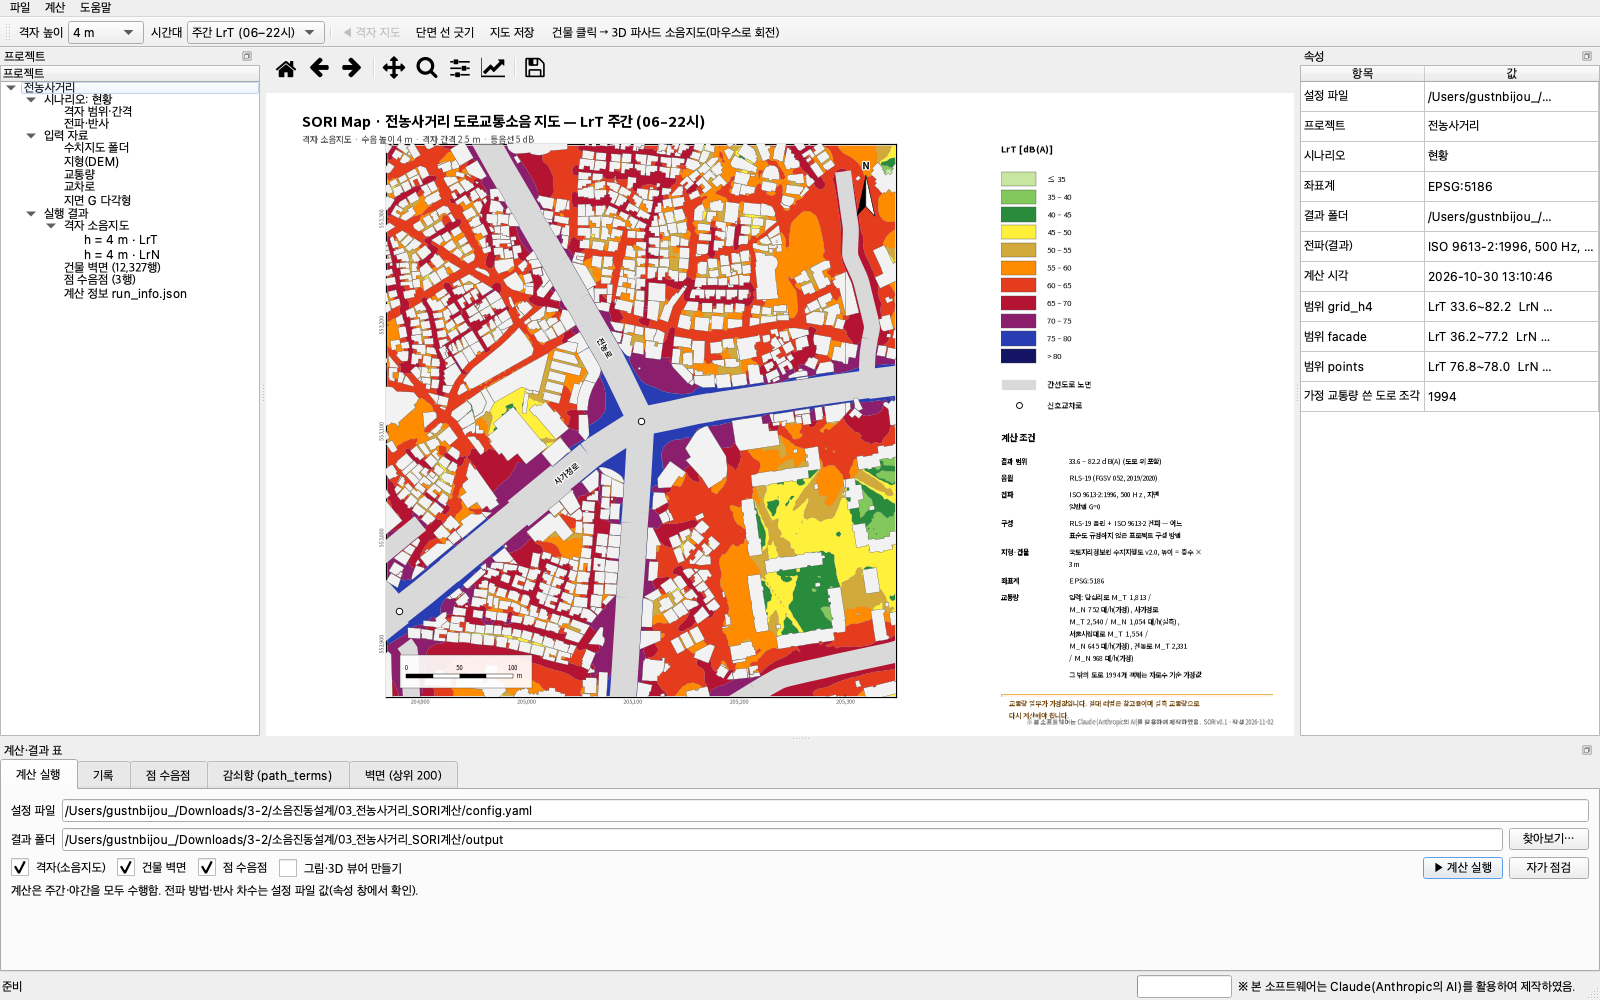
\includegraphics[width=\textwidth]{figures/gui_grid.png}
\caption{주 창 — 전농사거리 기본 계산 결과를 연 모습(격자 높이 4 m, 주간 LrT). 2026-11-02, 커밋 \f{2376a59} 화면을 화면 없이 그려 저장한 것}\label{fig:main}
\end{figure}

\begin{table}[h]\centering\small
\caption{화면 부분}\label{tab:parts}
\begin{tabularx}{\textwidth}{P{30mm}L}
\toprule
부분 & 내용 \\ \midrule
메뉴 \ui{파일} & 설정 파일 열기(Command/Ctrl+O), 결과 폴더 열기, 예제 불러오기(가상 교차로), 지도 저장(PNG·PDF, Command/Ctrl+S), 마지막 단면 보기, 결과 폴더를 파인더/탐색기로 보기, 끝내기 \\
메뉴 \ui{계산} & 계산 실행, 자가 점검 \\
메뉴 \ui{도움말} & SORI 정보(판, 적용 기준, AI 활용 고지) \\
도구 줄 & 격자 높이, 시간대(주간 LrT / 야간 LrN), \ui{◀ 격자 지도}, \ui{단면 선 긋기}, \ui{지도 저장…} \\
지도(가운데) & 격자 소음지도 / 3D 파사드 / 단면 지도. 위쪽 matplotlib 도구(처음·뒤·앞·이동·확대·여백·저장) \\
\ui{프로젝트}(왼쪽) & 시나리오·입력 자료·실행 결과 목록. 항목을 누르면 속성 창에 내용 \\
\ui{속성}(오른쪽) & 설정·결과 요약, 클릭한 격자점·건물·단면의 값 \\
\ui{계산·결과 표}(아래) & 탭: 계산 실행 / 기록 / 점 수음점 / 감쇠항(path\_terms) / 벽면(상위 200) \\
상태 줄 & 진행 상황 글, 마우스 좌표(X·Y), 진행 막대, AI 활용 고지 \\
\bottomrule
\end{tabularx}
\end{table}

PySide6 를 불러오지 못하면 단순 화면(tkinter)이 열린다. 단순 화면은 설정·결과 폴더 선택, 계산 실행, 결과 폴더 열기, 예제, 자가 점검만 있고 지도는 없다.

%% =====================================================================
\section{화면 사용법}

\subsection{설정 열기}
\begin{itemize}
\item \ui{파일}\menu\ui{설정 파일 열기…}로 \f{config.yaml} 을 고른다. 결과 폴더는 설정 파일 옆 \f{output} 으로 정해지고, 그 폴더에 결과가 있으면 지도에 바로 보인다.
\item 처음이면 \ui{파일}\menu\ui{예제 불러오기(가상 교차로)}. 앱 안의 가상 교차로(실제 지역 아님) 입력을 \f{문서/SORI/예제\_가상교차로} 에 복사해 연다.
\item 앱은 마지막에 연 설정과 결과 폴더를 짝으로 기억한다(사용자 폴더 \f{settings.json}). 다음에 켜면 그 설정이 열린다. 기억된 결과 폴더가 다른 설정으로 계산한 것이면(\f{run\_conditions.json} 의 \f{config\_path} 로 판단) 쓰지 않고 설정 옆 \f{output} 을 연다.
\item 계산 결과 폴더만 보려면 \ui{파일}\menu\ui{결과 폴더 열기…}. 이 경우 설정이 없어 격자 지도는 간단한 지도로 보이고 단면 계산은 할 수 없다.
\end{itemize}

\subsection{계산 실행}
\begin{enumerate}
\item \ui{계산 실행} 탭에서 \ui{결과 폴더}를 확인한다(\ui{찾아보기…}로 변경).
\item 계산 대상을 고른다: \ui{격자(소음지도)}, \ui{건물 벽면}, \ui{점 수음점}(설정에 점 파일이 있을 때), \ui{그림·3D 뷰어 만들기}(보고서 그림 \f{HQ\_*}·\f{noise3d.html}).
\item \ui{▶ 계산 실행}. 결과 폴더에 이미 파일이 있으면 덮어쓸지 묻는다. 계산은 주간·야간을 모두 수행하며 전파 방법·반사 차수는 설정 파일 값이다(속성 창에서 확인).
\item 진행은 상태 줄(지점 수, 남은 시간)과 \ui{기록} 탭에서 본다. 끝나면 결과가 지도와 표에 나온다. 계산 중에 창을 닫으면 끝낼지 묻는다.
\end{enumerate}
결과 폴더에는 계산 결과(7장) 외에 \f{config\_used.yaml}(사용한 설정 사본)과 \f{run\_conditions.json}(실행 일시·설정 경로·계산 대상·소요 시간·요약·앱 환경)이 함께 저장된다.

\subsection{격자 소음지도(보고서 수준)}
설정과 결과가 모두 열려 있으면 화면 지도는 보고서용 지도(\f{HQ\_grid\_*.png})와 같은 그림이다: 5 dB 등음선 채움, 간선도로 노면·건물·신호교차로·도로명, 방위표·축척, 범례·계산 조건·주의 문구(그림~\ref{fig:main}).
\begin{itemize}
\item 도구 줄에서 \ui{격자 높이}와 \ui{시간대}를 고른다.
\item 화면은 A3 틀을 창에 맞춰 줄여 보이므로 정보란 글자가 작다. 확대(돋보기)·이동 도구로 자세히 본다. 창 크기를 바꾸면 다시 그린다.
\item 격자점을 클릭하면 속성 창에 그 점의 좌표·지면고·높이·LrT·LrN·성분(직접음, 반사 차수별)이 나온다.
\end{itemize}

\subsection{건물 클릭 → 3D 파사드 소음지도}
\begin{figure}[h]\centering
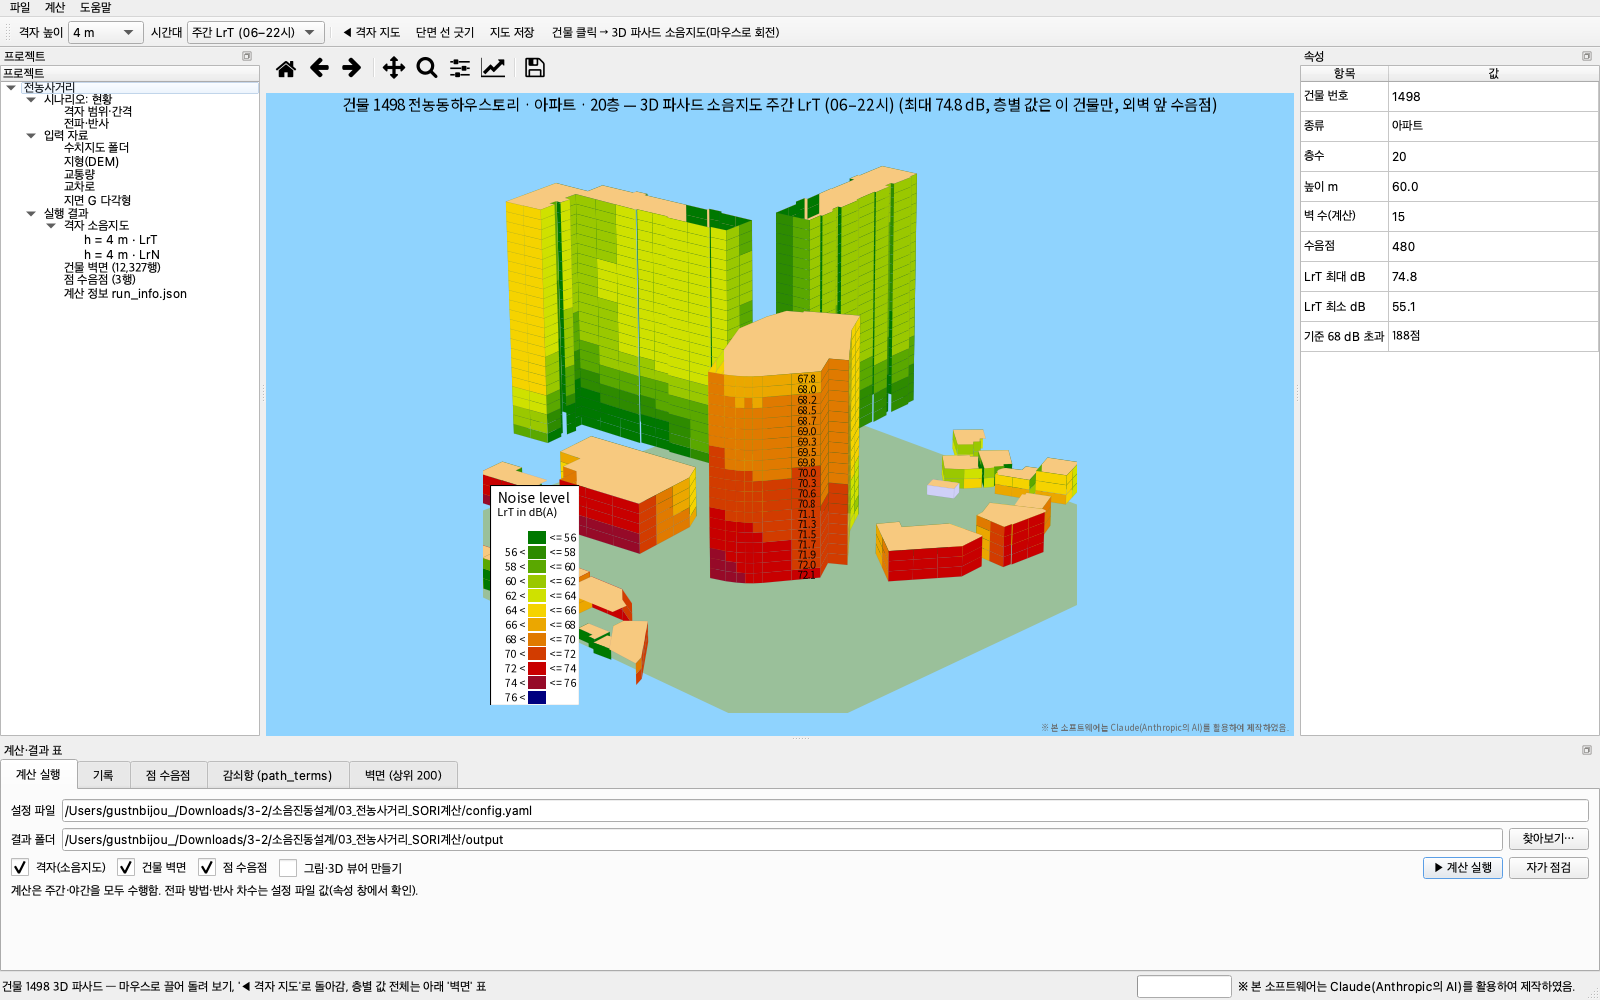
\includegraphics[width=0.92\textwidth]{figures/gui_facade3d.png}
\caption{건물 1498 클릭 — 3D 파사드 소음지도(주간 LrT, 2 dB 등급). 속성 창에 건물 정보와 기준 초과 수음점 수}\label{fig:facade}
\end{figure}
\begin{itemize}
\item 격자 지도에서 \textbf{건물을 클릭}하면 그 건물을 중심으로 반경 80 m 안의 건물을 그린 3D 파사드 소음지도가 나온다(그림 파일 \f{facade\_3d\_*.png} 와 같은 모양, 2 dB 등급).
\item 주변 건물도 벽면 결과가 있으면 층별 색으로 칠하고, 층별 값 글자는 클릭한 건물에만 붙인다. 마우스로 끌어 돌려 본다.
\item 클릭한 건물의 층별 값 전체는 아래 \ui{벽면} 표에 나온다.
\item 벽면 계산 반경(\f{receivers.facade.radius}) 밖 건물은 상태 줄에 ``벽면 계산 결과 없음''으로 표시된다.
\item \ui{◀ 격자 지도}로 돌아간다.
\end{itemize}

\subsection{단면(수직) 소음지도}
\begin{figure}[h]\centering
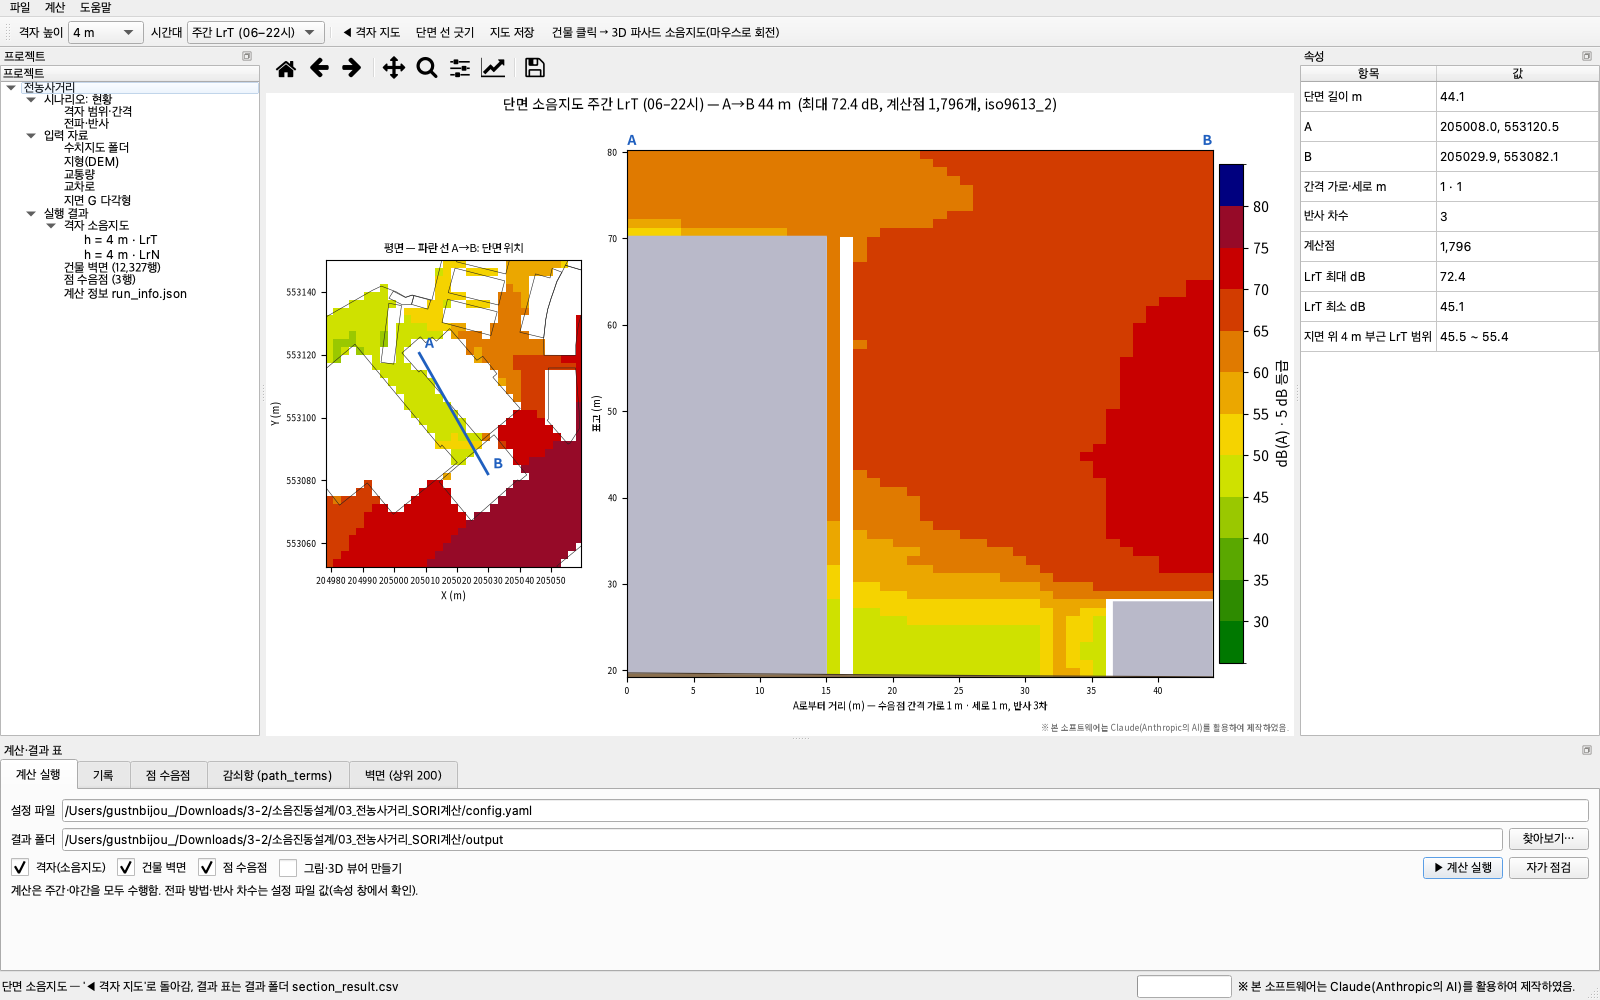
\includegraphics[width=0.92\textwidth]{figures/gui_section.png}
\caption{단면 소음지도 — A→B 44 m, 계산점 1,796개(반사 3차). 왼쪽 평면에 단면 위치, 회색은 건물 단면}\label{fig:section}
\end{figure}
\begin{enumerate}
\item 격자 지도에서 \ui{단면 선 긋기}를 누른다.
\item 시작점 A, 끝점 B 를 차례로 클릭한다. 계산이 백그라운드에서 돌고 진행이 상태 줄에 나온다.
\item 끝나면 거리 × 표고 단면 지도가 나온다. 지형과 건물 단면을 함께 그리며 건물 안(지붕 아래)·지면 아래는 계산하지 않는다.
\end{enumerate}
\begin{itemize}
\item 계산점 간격은 점 수가 약 4,000 개 안쪽이 되게 자동으로 정한다(가로 1 m, 세로 0.5 m 단위). 계산은 격자와 같은 함수·반사 차수(\f{max\_order\_grid})를 쓴다. 같은 위치의 지면 위 4 m 값이 격자 결과와 최대 0.007 dB 안에서 같음을 시험으로 확인했다.
\item 계산 시간 예: 전농사거리 180 m 단면, 계산점 약 3,200 개에 약 25초(macOS arm64).
\item 결과는 결과 폴더의 \f{section\_result.csv}, \f{section\_info.json}, 규칙 이름 사본(\f{…\_주야\_section.csv})에 저장된다. 다음에 결과 폴더를 열면 \ui{파일}\menu\ui{마지막 단면 보기}로 다시 본다.
\item \textbf{주의}: 음원(노면 위 0.5 m) 바로 위의 낮은 점은 근거리라 값이 매우 크게 나올 수 있다(전농사거리에서 최대 94.5 dB 관찰).
\item 단면 계산에는 설정 파일과 계산한 결과 폴더(모델 파일 \f{model\_rasters.npz})가 필요하다.
\end{itemize}

\subsection{지도 저장}
\ui{지도 저장…}(또는 \ui{파일}\menu\ui{지도 저장}, Command/Ctrl+S)으로 지금 보이는 지도(격자·3D 파사드·단면)를 PNG(200 dpi) 또는 PDF 로 저장한다. 확장자가 없거나 다르면 PNG 로 저장한다. 기본 이름은 결과 파일명 규칙을 따른다(7.1절). 예:
\begin{itemize}
\item \f{전농사거리\_현황-ISO\_주간\_grid\_h4m.png}
\item \f{전농사거리\_현황-ISO\_주간\_facade\_3D\_건물1498.png}
\item \f{전농사거리\_현황-ISO\_주간\_section.png}
\end{itemize}
그림 안에는 AI 활용 고지가 들어간다.

\subsection{자가 점검}
\ui{자가 점검} 단추(또는 \ui{계산}\menu\ui{자가 점검})는 이 PC 에서 앱이 올바로 계산하는지 확인한다(1–2분).
\begin{itemize}
\item 좌표 변환: EPSG 5186·5179·4326 사이 변환 8 항목을 기준값과 비교.
\item 기준 사례: 앱 안의 가상 교차로를 계산해 기준값과 비교. 허용 오차 0.01 dB·m 단위 값(프로젝트 임의 설정).
\item 결과는 상태 줄(``자가 점검 통과 — 기준 사례 최대 차이 …'')과 보고서 \f{문서/SORI/selfcheck\_report.json}.
\end{itemize}
지금까지 macOS 로컬·Actions macOS·Actions Windows(화면 없이) 모두 최대 차이 5e-11 dB 로 통과했다.

%% =====================================================================
\section{전농사거리 기본 계산 폴더}

수업 대상지(전농사거리)를 바로 계산할 수 있게 입력과 설정을 모은 폴더가 저장소 밖에 있다: \f{소음진동설계/03\_전농사거리\_SORI계산}.

\begin{table}[h]\centering\small
\caption{폴더 구성}\label{tab:jn}
\begin{tabularx}{\textwidth}{P{40mm}L}
\toprule
경로 & 내용 \\ \midrule
\f{config.yaml} & 기본 계산 설정. 입력은 결과보고서 6.8절(사가정로 50 km/h)과 같고 반사는 SORI 현재 기본값(3차) \\
\f{traffic.csv} & 계산에 쓰는 교통량 = \f{traffic/A\_현장계수\_50kmh.csv} 사본 \\
\f{traffic/} & 교통량 자료 A(기본, 사가정로 2026-10-22 현장 계수 + 나머지 가정)·B(사가정로 30 km/h)·C(기준선 가정값)·D(산정근거 문서) \\
\f{points.csv} & 2026-10-22 현장 측정점(P1·P2·P2c) \\
\f{data/map/} & 국토지리정보원 수치지형도 v2.0(2025) 9도엽 \\
\f{output/} & 계산 결과 \\
\f{output\_2026-10-29\_이전엔진/} & 엔진 변경 전 결과(보고서와 1e-10 dB 이내로 같음) 보관 \\
\bottomrule
\end{tabularx}
\end{table}

\begin{itemize}
\item 앱을 처음 쓸 때 이 폴더의 \f{config.yaml} 을 열고 \ui{▶ 계산 실행}. 기본값(반사 3차)으로 약 21분 걸린다(macOS arm64, 앱 \f{--run} 실측 21분 28초). 격자 2.5 m × 25,719 점, 건물 벽면 12,327 점, 측정점 3 점.
\item 반사 기본값이 2026-10-29 에 3차로 바뀌어 결과보고서 값(1·2차)과 다르다. 보고서 조건 재현 방법은 \f{config.yaml} 주석에 있다.
\item 다른 교통량으로 계산하려면 원하는 파일을 \f{traffic.csv} 로 복사하거나 \f{input.traffic.path} 를 바꾼다.
\end{itemize}

%% =====================================================================
\section{새 지역 계산 절차(명령행)}

\begin{enumerate}
\item 작업 폴더 만들기: \f{python -m sori init 폴더} → \f{config\_example.yaml} 을 \f{config.yaml} 로 바꾼다.
\item 수치지도 넣기: 국토정보플랫폼에서 받은 수치지형도 v2.0(SHP) 압축을 \f{data/map/} 아래에 도엽별로 푼다(하위 폴더 자동 탐색, 여러 도엽 자동 병합). 쓰는 층: B001(건물), A002(도로), F001(등고선), F002(표고점).
\item DEM(선택): \f{input.dem.path} 에 GeoTIFF/IMG. 좌표계는 파일에서 읽어 자동 변환.
\item 계산 중심: \f{receivers.center: [x, y]}(EPSG:5186).
\item 교통량 서식: \f{python -m sori template -c config.yaml} → \f{traffic\_template.csv} 에 값 입력 → \f{traffic.csv} 로 저장.
\item 교차로 확인(선택): \f{traffic\_template\_junctions\_auto.csv} 의 자동 판정(type)을 검토·수정해 \f{input.junctions.path} 로 지정.
\item 실행: \f{python -m sori all -c config.yaml}(모델 구축 → 계산 → 그림). 나눠 하려면 \f{build}, \f{run}(\f{--grid}, \f{--facade}, \f{--points}), \f{plot}.
\item 결과 확인: \f{output/}(7장). 앱으로 \f{config.yaml} 을 열어 지도로 봐도 된다.
\end{enumerate}
가상 자료로 연습: \f{python tools/make\_synthetic\_data.py examples/synthetic} 후 그 폴더에서 \f{python -m sori all -c config.yaml}.

%% =====================================================================
\section{입력 자료 서식}
CSV 는 UTF-8 또는 CP949 로 읽는다(읽은 인코딩은 기록에 남음). 따옴표 없는 쉼표로 칸 수가 늘어난 행은 줄 번호와 함께 오류를 낸다.

\subsection{교통량 \f{traffic.csv}}
\begin{longtable}{P{30mm}P{10mm}P{112mm}}
\caption{교통량 열(●필수, △둘 중 하나)}\label{tab:traffic}\\
\toprule 열 & 필수 & 설명 \\ \midrule\endfirsthead
\toprule 열 & 필수 & 설명 \\ \midrule\endhead
\f{key} & ● & 도로명(예: 사가정로) 또는 수치지도 UFID \\
\f{key\_type} & & \f{name}(기본) 또는 \f{ufid}. UFID 행이 도로명 행보다 우선 \\
\f{road\_type} & & RLS-19 표 2: \f{autobahn}, \f{bundesstrasse}, \f{landesstrasse}, \f{gemeinde}(빈칸 보충용) \\
\f{DTV} & △ & 일평균 교통량(대/일, 양방향 합) \\
\f{M\_day}, \f{M\_night} & △ & 시간당 교통량(대/h, 양방향 합). 비우면 DTV × 표 2 계수. DTV 없이 한쪽만 넣으면 기본은 오류(문제 행을 모두 나열). \f{input.traffic.missing\_m: estimate} 이면 표 2 주·야 계수 비율로 보충(가정값, 서울 간선에서 야간 과소 추정 가능) \\
\f{p1\_day} … \f{p2\_night} & & Lkw1·Lkw2 비율 \%. 비우면 표 2 표준값 \\
\f{v\_pkw}, \f{v\_lkw} & & 차종별 속도 km/h(30 미만은 30 적용) \\
\f{surface} & & 노면: \f{ref}, \f{AC11}, \f{SMA5\_8}, \f{SMA8\_11}, \f{PA11}, \f{PA8}, \f{Waschbeton}, \f{LGA}, \f{LOA}, \f{SMA\_LA8}, \f{DSH\_V5}, \f{pflaster\_even}, \f{pflaster\_other} \\
\f{grade} & & 도로별 종단경사 \% 직접 지정(깎거나 쌓은 도로) \\
\f{basis} & & 교통량 근거 \f{measured}/\f{assumed}(빈칸이면 unspecified) \\
\f{dir\_split\_fwd}, \f{dir\_basis} & & 디지타이즈 방향 비율(0–1). UFID 행이고 \f{dir\_basis = measured} 일 때만 적용, 그 밖은 0.5 \\
\f{note} & & 출처 메모 \\
\bottomrule
\end{longtable}
교통량 파일에 없는 도로는 \f{fallback\_dtv\_by\_lanes}(차로수별 가정값, 기본 1차로 1,000 … 6차로 40,000 대/일)를 쓰고 \f{traffic\_used.csv} 에 \f{traffic\_src = fallback} 으로 표시된다.

\subsection{그 밖의 입력(선택)}
\begin{itemize}
\item \textbf{교차로 \f{junctions.csv}}: \f{x, y, type}. type 은 \f{signal}(KKT 3), \f{roundabout}(2), \f{other}(0). 반경 30 m 안의 자동 교차점 군집에 적용.
\item \textbf{다공성 지면}: 녹지 폴리곤(SHP/GPKG)을 \f{input.ground.soft\_polygons} 에 지정하면 그 범위의 G = \f{soft\_G}(기본 1). 기본 지면은 G = 0(포장).
\item \textbf{도로별 확인값 \f{roads\_override.csv}}(\f{input.road\_override.path}): \f{ufid}, \f{lanes\_fwd}, \f{lanes\_bwd}, \f{oneway\_dir}(+1/−1), \f{lanes\_basis}, \f{oneway\_dir\_basis}, \f{note}. 서식 예: \f{sori/templates/roads\_override\_example.csv}.
\item \textbf{점 수음점 \f{points.csv}}(\f{receivers.points.path}): \f{point\_id}, \f{x}, \f{y}(계산 좌표계), \f{h}(지면 위 높이, 빈칸이면 \f{default\_height}, 그것도 없으면 건너뜀). 건물 안·모델 범위 밖 점은 계산하지 않고 \f{note} 에 적는다.
\end{itemize}

\subsection{주요 설정 \f{config.yaml}}
\begin{longtable}{P{48mm}P{22mm}P{82mm}}
\caption{자주 바꾸는 설정(기본값은 \f{sori/config.py})}\label{tab:cfg}\\
\toprule 항목 & 기본값 & 의미 \\ \midrule\endfirsthead
\toprule 항목 & 기본값 & 의미 \\ \midrule\endhead
\f{project.name}, \f{scenario} & 소음지도, 현황 & 파일명 규칙의 프로젝트·시나리오 칸 \\
\f{project.output\_dir} & output & 결과 폴더(설정 파일 기준 상대경로) \\
\f{propagation\_method} & iso9613\_2 & 전파 방법. \f{rls19} = RLS-19 3.5·3.6. 한 결과 폴더에는 한 방법의 결과만(섞이면 실행 중단) \\
\f{reflection.max\_order\_grid / \_facade / \_point} & 3 / 3 / 3 & 반사 차수 0–3. 3차는 2차보다 약 6배 느림(전농사거리 표본). 2026-10-29 이전 기본 1/2/2 \\
\f{reflection.own\_facade} & last & 수음점이 놓인 외벽의 반사 제외 범위. \f{last} = 마지막 반사만, \f{all} = 모든 반사 순서(이전 동작) \\
\f{reflection.rho} / \f{D\_RV} & 0.8 / 0.5 dB & 반사 손실(iso9613\_2 의 ρ / rls19 의 회당 dB) \\
\f{receivers.grid.step}, \f{heights} & 5 m, [4.0] & 격자 간격, 높이 목록(여러 개 = 3D 격자) \\
\f{receivers.facade.radius} & 230 m & 벽면 계산 반경 \\
\f{propagation.max\_dist\_main / minor} & 300 / 150 m & 음원 탐색 거리(간선 / 이면도로) \\
\f{input.ground.method} & general & ISO 7.3.1 일반법, \f{alternative} = 7.3.2(다공성 지면 전제) \\
\f{propagation.terms\_csv} & false & 점 수음점 감쇠항별 중간값 \f{path\_terms.csv} \\
\f{input.junctions.dk\_rule} & nearest & 교차로 보정 기준 교차점(\f{nearest\_signal} = 가까운 신호교차로 값과 큰 쪽) \\
\f{plots.limits} & 없음 & 기준 초과 지도의 기준값(예: \f{\{LrT: 68, LrN: 58\}}) \\
\bottomrule
\end{longtable}
그 밖의 설정(차로폭, 홀수 차로 규칙, 음원 높이 기준 지면 등)은 Technical Manual 과 \f{README.md} 5절에 있다.

%% =====================================================================
\section{출력 파일}

\subsection{파일명 규칙}
고정 이름 파일과 함께 \f{\{프로젝트\}\_\{시나리오\}-\{ISO|RLS\}\_\{주간|야간|주야\}\_\{grid|facade|section\}[부가]} 이름의 사본을 만든다(\f{project.file\_naming: false} 이면 만들지 않음). 방법 표시는 \f{propagation\_method} 에서 자동으로 붙고, 두 시간대를 함께 담은 CSV 는 \f{주야}, 격자 높이·지도 종류는 부가(\f{\_h4m}, \f{\_exceed\_h4m}, \f{\_building})로 붙는다. 만든 목록은 \f{run\_info.json} 의 \f{file\_naming}.

\subsection{결과 폴더의 파일}
\begin{longtable}{P{57mm}P{95mm}}
\caption{출력 파일}\label{tab:out}\\
\toprule 파일 & 내용 \\ \midrule\endfirsthead
\toprule 파일 & 내용 \\ \midrule\endhead
\f{grid\_result.csv}, \f{grid\_LrT\_h4m.tif} … & 격자 결과(높이별). GeoTIFF 는 QGIS 에서 바로 열림 \\
\f{facade\_result.csv} & 벽면 결과(층별). \f{LrT\_cmp} = RLS-19 3.1 올림값, \f{LrT\_direct/refl1/refl2/refl3} = 성분 \\
\f{point\_result.csv}, \f{point\_levels\_for\_comparison.csv} & 점 수음점 결과, 측정값 비교용 표 \\
\f{section\_result.csv}, \f{section\_info.json} & 단면 결과(화면에서 계산했을 때) \\
\f{HQ\_*.png / .pdf} & 보고서·발표용 A3 지도(300 dpi + 벡터 PDF): 격자, 기준 초과, 벽면 색 띠, 건물별 평가도(주·야) \\
\f{noise3d.html} & 3D 웹 뷰어(지형 위 격자 + 벽면 층별). 더블클릭해 브라우저로 열기, 인터넷 없이 동작 \\
\f{*.png} & 확인용 간이 그림(격자, 파사드 평면, 파사드 3D) \\
\f{sources.csv}, \f{source\_lines.csv} & 음원 점별 LW′·보정값, 도로 객체별 음원선 배치 근거 \\
\f{path\_terms.csv} & (\f{terms\_csv: true}) 점 수음점 경로별 감쇠항 \\
\f{segment\_check.csv} & 구간 길이 진단(RLS-19 3.2 주석, 결과값에 영향 없음) \\
\f{traffic\_used.csv}, \f{junctions\_used.csv} & 실제 사용한 교통량·교차로 판정(보고서 근거자료) \\
\f{build\_info.json}, \f{run\_info.json} & 모델 규모, 가정값 사용 수, 계산 조건(전파 방법·식·반사 차수) \\
\f{config\_used.yaml}, \f{run\_conditions.json} & 앱이 남기는 사용 설정 사본과 실행 조건 \\
\f{model\_rasters.npz}, \f{*.gpkg} & 모델 파일(단면 계산·화면 지도에 씀) \\
\bottomrule
\end{longtable}

\subsection{지표 읽는 법}
LrT 는 주간(06–22시), LrN 은 야간(22–06시) RLS-19 평가레벨이다. 둘 다 A 가중 등가소음도이며 교차로 보정·반사를 포함한다. 기준과 비교할 때는 RLS-19 3.1 에 따라 정수로 \textbf{올린} 값(\f{LrT\_cmp})을 쓴다.

%% =====================================================================
\section{계산 시간}
단일 코어 기준 수음점 1개당 수 ms(가상 자료)–수십 ms(도심)이고 numba 가 CPU 코어를 모두 쓴다. 전농사거리 기본 계산은 약 21분(4장). 빠른 시험은 \f{grid.step} 을 10 m 로, 반사 차수를 1 로 낮춘다. 앱을 처음 실행하거나 새 판으로 바꾼 뒤 첫 계산은 컴파일 때문에 1분 정도 더 걸린다.

%% =====================================================================
\section{문제 해결}

\begin{longtable}{P{52mm}P{100mm}}
\caption{자주 생기는 문제}\label{tab:faq}\\
\toprule 증상 & 원인과 대처 \\ \midrule\endfirsthead
\toprule 증상 & 원인과 대처 \\ \midrule\endhead
macOS ``확인되지 않은 개발자'' / ``열 수 없음'' & 서명·공증하지 않은 앱. 2.4절 절차로 한 번 허용 \\
Windows ``PC 보호'' 창 & 같은 이유. \ui{추가 정보}\menu\ui{실행}(실제 PC 미확인 \chk) \\
\f{SORI.exe} 만 꺼내 실행하면 실행되지 않음 & zip 을 폴더째 풀지 않음(\f{\_internal} 없음). 폴더째 다시 풀기 \\
Intel Mac 에서 열리지 않음 & 앱은 Apple Silicon(arm64) 전용 \\
첫 계산이 느림 & numba 컴파일(1분 정도). 다음부터는 캐시 사용 \\
다른 프로젝트 결과가 지도에 보임 & 결과 폴더가 다른 설정의 것. 설정을 다시 열거나 \ui{결과 폴더}를 바꿈 \\
다른 전파 방법의 결과가 있다며 계산 중단 & 한 결과 폴더에는 한 전파 방법만. \f{project.output\_dir} 를 바꿈 \\
``결과 파일을 덮어쓸까요?'' & 결과 폴더에 이미 파일이 있음. 보관하려면 다른 폴더를 고름 \\
교통량 오류(M 한쪽만 입력) & \f{DTV} 나 두 \f{M} 을 모두 넣거나 \f{missing\_m: estimate}(가정값) \\
CSV 칸 수 오류 & 따옴표 없는 쉼표. 메모 칸을 따옴표로 묶음 \\
건물 클릭 시 ``벽면 계산 결과 없음'' & 벽면 계산 반경 밖이거나 벽면을 계산하지 않음. \f{receivers.facade.radius} 를 키우고 \ui{건물 벽면}을 골라 다시 계산 \\
\ui{단면 선 긋기}가 오류 & 설정 파일과 계산한 결과 폴더(\f{model\_rasters.npz})가 열려 있어야 함. 단면 선 1 m 미만, 모델 범위 밖도 오류 \\
단면에서 도로 바로 위 값이 매우 큼 & 음원 근거리 값(오류 아님, 4.5절) \\
지도 정보란 글자가 겹침 & 교통량 설명이 길면 주의 문구가 AI 고지와 겹침(알려진 문제) \\
자가 점검 실패 & \f{문서/SORI/selfcheck\_report.json} 의 실패 항목 확인. 좌표 변환 실패는 PROJ 자료 문제 가능성 \\
\bottomrule
\end{longtable}

%% =====================================================================
\appendix
\section{명령어 요약}
\begin{Verbatim}
python -m sori init 폴더                 # 작업 폴더·설정 예제
python -m sori template -c config.yaml   # 교통량·교차로 서식
python -m sori all -c config.yaml        # build → run → plot
python -m sori run -c config.yaml --points   # 점 수음점만
python -m pytest -q tests                # 시험(236 통과·1 xfailed, 2026-11-02)
python tools/check_baseline.py           # 전농사거리 기준선 비교(약 1분)
python tools/reference.py make|compare   # 기준 사례 기준값 만들기·비교
\end{Verbatim}

\section{웹 화면(Streamlit)}
\f{pip install -r requirements.txt} 후 \f{run\_app.bat}(Windows) 또는 \f{./run\_app.sh}(Mac/Linux), 또는 \f{streamlit run app.py}. 브라우저에서 1. 지도 자료(수치지도 zip 업로드·폴더·예제) → 2. 위치·범위(지도에서 교차로 클릭) → 3. 교통량(아는 값만 입력) → 4. 계산·결과(빠른 미리보기·표준은 반사 1차, 정밀은 격자·벽면 3차). 결과와 설정은 \f{projects/프로젝트이름/} 에 저장된다. 배경지도는 인터넷이 필요하다. 웹 화면은 앱에 들어 있지 않다.

\section{용어}
\begin{tabularx}{\textwidth}{P{30mm}L}
\toprule
LrT / LrN & 주간 / 야간 평가레벨(RLS-19), dB(A) \\
LW′ & 음원선 1 m 당 음향파워레벨 \\
파사드(벽면) 수음점 & 건물 외벽 앞 5 cm, 층별 \\
허상음원 & 반사면에 대칭으로 둔 가상 음원(반사 계산) \\
DTV, M & 일평균 교통량, 시간당 교통량 \\
Pkw, Lkw1, Lkw2 & 승용차, 트레일러 없는 화물차·버스, 트레일러 화물차(이륜차는 방출상 Lkw2) \\
\bottomrule
\end{tabularx}

\end{document}
